\documentclass[french,pdf]{beamer}

% spécifie la langue utilisée
\usepackage[english,main=french]{babel}

% permet d'entrer des caractères utf8
\usepackage[utf8]{inputenc}

% permet d'afficher correctement les caractères utf8
\usepackage[T1]{fontenc}

% permet d'ajouter des images présent dans le fichier
\usepackage{graphicx}
\graphicspath{ {./rsc/} }

% permet d'ajouter des tableaux
\usepackage{array,multirow,makecell}
\setcellgapes{1pt}
\makegapedcells
\newcolumntype{R}[1]{>{\raggedleft\arraybackslash }b{#1}}
\newcolumntype{L}[1]{>{\raggedright\arraybackslash }b{#1}}
\newcolumntype{C}[1]{>{\centering\arraybackslash }b{#1}}
\newcommand\tabitem{~~\llap{\textbullet}~~}

% permet de dessiner des arbres
\usepackage{dirtree}

% ajout du numéro de diapo dans les symboles de manipulation
\addtobeamertemplate{navigation symbols}{}{ \hspace{0.5cm}    \usebeamerfont{footline}%
    \insertframenumber / \inserttotalframenumber }

%  définie le thème du diapo
\usetheme{Hannover}
\useoutertheme[height=0pt,left]{sidebar}
\usecolortheme{seahorse}
\setbeamercolor*{titlelike}{parent=structure}
\useinnertheme{circles}
\setbeamertemplate{frametitle}[default][left]

\begin{document}
% permet de ne pas afficher le plan
{
\setbeamercolor{section in sidebar}{fg=structure.fg!20!white}
\setbeamercolor{subsection in sidebar}{fg=structure.fg!20!white}
\begin{frame}
  \begin{minipage}{0.45\textwidth}
    \begin{flushleft}
      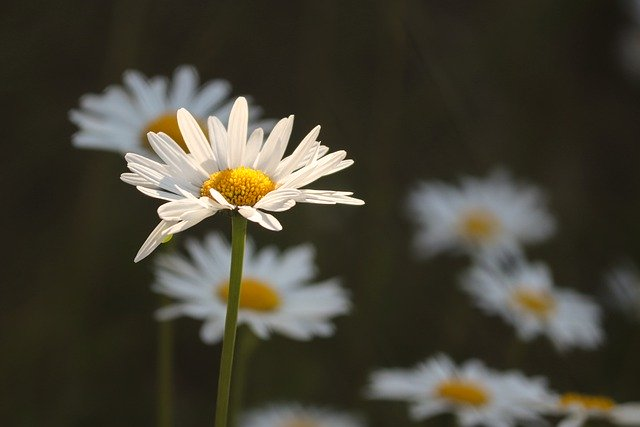
\includegraphics[width=2.5cm]{img.jpg}
    \end{flushleft}
  \end{minipage}
  \begin{minipage}{0.53\textwidth}
    \begin{flushright}
      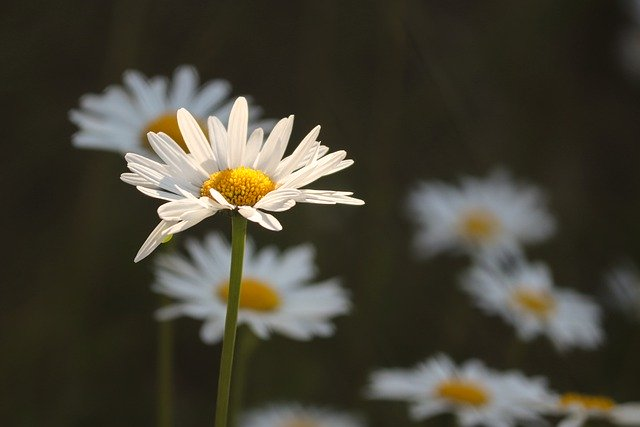
\includegraphics[width=2cm]{img.jpg}
    \end{flushright}
  \end{minipage}

  \newcommand{\HRule}{\rule{\linewidth}{0.1mm}}
  \center

  \textsc{\Large Diplôme}\\
  \textsc{\Large Spécialité}\\
  \textsc{\large Stage du ../../.... au  ../../....}\\

  \HRule \\[0.1cm]
  { \Large \bfseries Titre du stage}\\[0.1cm]
  \HRule \\[0.3cm]

  \begin{minipage}{0.4\textwidth}
    \begin{flushleft} \large
      \emph{Réalisé par:}\\
      \textsc{...}
    \end{flushleft}
  \end{minipage}
  \begin{minipage}{0.4\textwidth}
    \begin{flushright} \large
      \emph{Tuteur en entreprise:} \\
      \textsc{...} \\ [0.1cm]
      \emph{Tutrice universitaire:} \\
      \textsc{...} \\
    \end{flushright}
  \end{minipage}
  \vfill
\end{frame}
}

% permet de ne pas afficher le plan
{
\setbeamercolor{section in sidebar}{fg=structure.fg!20!white}
\setbeamercolor{subsection in sidebar}{fg=structure.fg!20!white}
\begin{frame}{Sommaire}
  \begin{columns}[t]
    \begin{column}{5cm}
      \tableofcontents[sections={1-3}, hideothersubsections]
    \end{column}
    \begin{column}{5cm}
      \tableofcontents[sections={4-6}, hideothersubsections]
    \end{column}
  \end{columns}
\end{frame}
}

\section{Introduction}
\begin{frame}
  \vfill
  \centering
  \begin{beamercolorbox}[sep=8pt,center,shadow=true,rounded=true]{title}
    \usebeamerfont{title}\insertsectionhead\par%
  \end{beamercolorbox}
  \vfill
\end{frame}

\section{section}
 % permet de ne pas afficher le plan
 {
  \setbeamercolor{section in sidebar}{fg=structure.fg!20!white}
  \setbeamercolor{subsection in sidebar}{fg=structure.fg!20!white}
  \begin{frame}
    \vfill
    \centering
    \begin{beamercolorbox}[sep=8pt,center,shadow=true,rounded=true]{title}
      \usebeamerfont{title}\insertsectionhead\par%
    \end{beamercolorbox}
    \vfill
    \begin{columns}[t]
      \begin{column}{5cm}
        \tableofcontents[sections={1-3},currentsection, hideothersubsections]
      \end{column}
      \begin{column}{5cm}
        \tableofcontents[sections={4-6},currentsection,hideothersubsections]
      \end{column}
    \end{columns}
  \end{frame}
 }

\subsection{subsection}
\begin{frame}{subsection}
  \begin{itemize}
    \item item1 : aaa
    \item item2 : aaa
  \end{itemize}
  \begin{center}
    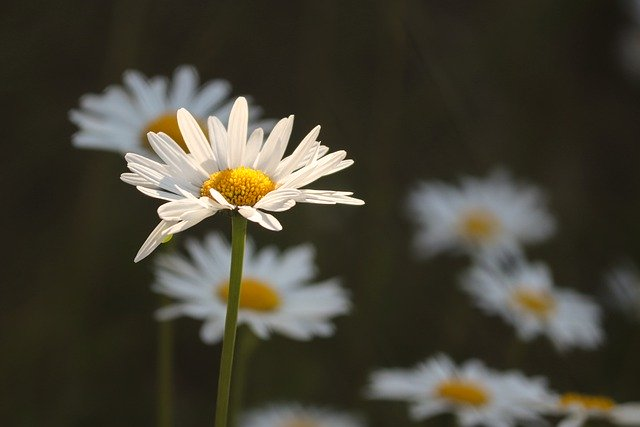
\includegraphics[scale=0.3]{img.jpg}
  \end{center}
\end{frame}

\section{Bilan}
\begin{frame}
  \vfill
  \centering
  \begin{beamercolorbox}[sep=8pt,center,shadow=true,rounded=true]{title}
    \usebeamerfont{title}\insertsectionhead\par%
  \end{beamercolorbox}
  \vfill
\end{frame}

\section{Conclusion}
\begin{frame}
  \vfill
  \centering
  \begin{beamercolorbox}[sep=8pt,center,shadow=true,rounded=true]{title}
    \usebeamerfont{title}\insertsectionhead\par%
  \end{beamercolorbox}
  \vfill
\end{frame}
\end{document}
